\documentclass[a4paper]{scrartcl}

\usepackage[utf8]{inputenc}
\usepackage[english]{babel}
\usepackage{lmodern}
\usepackage[T1]{fontenc}
\usepackage{booktabs}
\usepackage{multirow}
\usepackage{wrapfig}


% PAKETE
\usepackage{siunitx}
\usepackage{graphicx}
\usepackage{placeins}
\usepackage{longtable}
\usepackage{enumitem}
\usepackage{bbm}
%\usepackage{sidecap}


\usepackage{amssymb} % math symbols
\usepackage{amsmath} % ams
\usepackage{amsfonts} % mathmatical fonts

% caption indenting
 \usepackage[format=plain,indention=0em,labelfont=bf,margin=1em]{caption}
 \usepackage{subfig} %subfigures ^^
\usepackage[protrusion=true,expansion=true]{microtype} % denser font, "-" behind line
\usepackage{esint} % nicer double and triple integrals
\usepackage{fancyhdr} % fancy headers
\usepackage[colorlinks=true,linkcolor=black,citecolor=black,filecolor=black,urlcolor=black]{hyperref}



% EINSTELLUNGEN
\sisetup{seperr,repeatunits=false}
\numberwithin{equation}{section}
\numberwithin{figure}{section}
\numberwithin{table}{section}

% EIGENE FUNKTIONEN
\newcommand{\re}{\operatorname{Re}}
\newcommand{\im}{\operatorname{Im}}
\newcommand{\gquote}[1]{\glqq #1 \grqq}

\newcommand{\eq}[2]{\begin{equation}#1\label{#2}\end{equation}}
\newcommand{\eqand}[0]{\hspace{.25cm} \bigwedge \hspace{.25cm}}
\newcommand{\grafik}[2]{\begin{figure}[h]\centering \includegraphics[width=10cm]{#1.eps} \caption{#2} \label{#1} \end{figure} }
\newcommand{\grafikq}[3]{\begin{figure}[h]\centering \includegraphics[width=10cm]{#1.eps} \caption[#2]{#3} \label{#1} \end{figure} }
\newcommand{\tbl}[3]{\begin{table}[h]\caption{#1}\label{#2}\begin{center}#3\end{center}\end{table}}
\newcommand{\Abbildung}[1]{\textsl{Abbildung \ref{#1}}}
\newcommand{\AbbildungI}[1]{\textsl{(Abbildung \ref{#1})}}
\newcommand{\Tabelle}[1]{\textsl{Tabelle \ref{#1}}}
\newcommand{\TabelleI}[1]{\textsl{(Tabelle \ref{#1})}}
\newcommand{\Formel}[1]{(\ref{#1})}
\renewcommand{\d}{\mathrm{d}}
\newcommand{\ve}[1]{\mathbf{ #1} }

\title{Ma 12: Magneto-optic Kerr effect and Magnetic Anisotropy}
\subtitle{Tutor: B. Lewitz}
\author{Benjamin Huber, Carolin Wille}
\date{November 21, 2011}

\begin{document}
\thispagestyle{empty}
\maketitle
\tableofcontents
\clearpage


\section{Introduction}
The magneto-optic Kerr effect (MOKE) describes the changes in the polarization of light, which is reflected from the surface of a magnetic material. Therefore it can be used to analyze magnetic properties, such as the structure of magnetic domains or the phenomenon of hysteresis effects. It has a great application in magneto-optic data storage like in magneto-optic discs, which are written magnetically and read out optically making use of the Kerr effect. The Kerr effect is also used in Kerr microscopes, which directly show the structure of magnetic domains.

\subsection{Magneto-optic Kerr effect}
The magneto-optic Kerr effect is a quantum mechanical scattering effect. However, it can be qualitatively understood in the picture of classical electrodynamics. Therefore, we consider a light-wave, that is reflected from a surface. During the reflection process it
 penetrates into the material, before it is emitted again. During the time, the wave spends in the solid, the dielectric displacement $\ve D $ has to be considered instead of the electric field $\ve E$. The quantities are related via
\eq{\ve D_i = \epsilon_{ij} E_j \;, } {DE}
where $ \epsilon_{ij}$ is the permittivity tensor, that reduces to a scalar for isotropic materials. In magnetized materials, the tensor $\epsilon_{ij}$ decomposes into a real isotropic ($\alpha_{ij}$) and an imaginary totally antisymmetric ($\beta_{ij}$) contribution
\eq{\epsilon_{ij} = \epsilon_0 \alpha_{ij} + i \beta_{ij} \; . }{eps}
As the antisymmetric tensor $\beta_{ij}$ has vanishing diagonal entries, it can be expressed in terms of a cross-product with the so called gyration vector, that can be identified in a classical picture with the direction of the magnetic field $\ve j$. Equation \Formel{DE} can then be written as
\eq{\ve D = \epsilon_0 \ve E - i \epsilon_0 Q \ve j \times \ve E \; , }{DEJ}
where $\epsilon_0$ is the vacuum permittivity and $Q$ is a complex material constant, that is approximately proportional to the magnetization. The cross-product in equation \Formel{DEJ} describes a rotation around the magnetization axes by $\pi/2$, that can be described as a Lorentz force, which is acting on the electrons, that are oscillating in the material due to the periodic excitation of the incoming wave. However, the magnetic field, which would cause a Lorentz force needed to describe the rotation deviates significantly in orders of magnitutde when compared to the real magnetic field. Therefore this classical picture has to be used with caution.

A further analysis of the Maxwell equation for this problem \cite{book} leads to the conclusion of different refraction indices and amplitudes for left and right circular polarized light. As linear polarized light is nothing but a superposition of these two, it becomes clear, that its direction is rotated as a result of the phase shift between the two components and is furthermore polarized elliptically due to the different intensities (see Fig. \ref{fug:kerr}).



\begin{figure} 
 \centering
\subfloat[][Kerr and Faraday Effect]
{         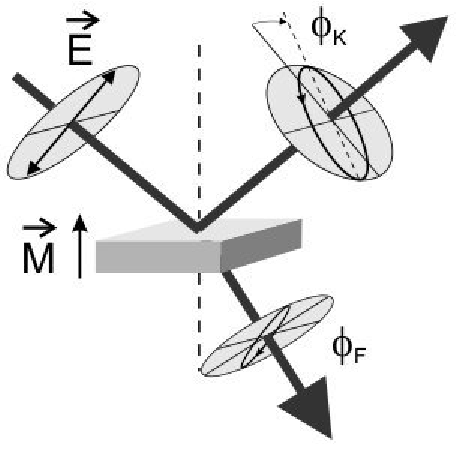
\includegraphics[width=0.4\linewidth]{img/kerrpic.pdf}
       
}
% \hfill
\subfloat[][Types of MOKE]
         {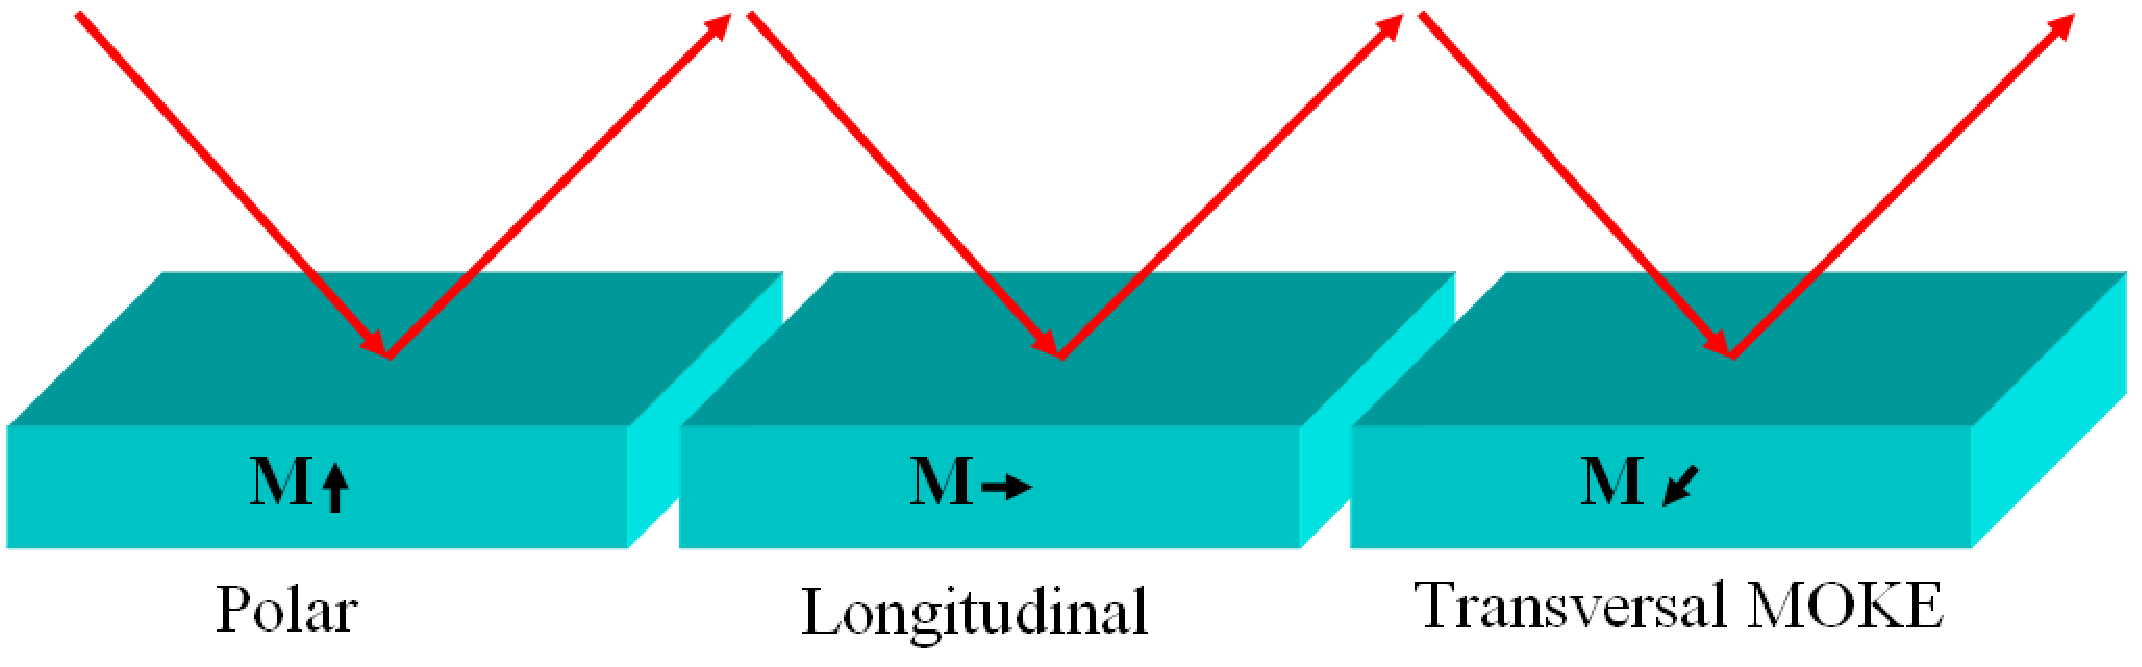
\includegraphics[width=0.6\linewidth]{img/moke.pdf}}

\caption{
\small $\ve a)$ Schematic description of the Kerr effect (polar) characterized by the Kerr angle $\phi_K$. The same effect occurring for the transmission of light is called Farrady effect \cite{dissert}. $\ve b)$ According to the direction of the magnetization of the sample $\ve M$ and the incidence plane three different types of MOKEs are characterized. 
Source: \url{http://en.wikipedia.org/wiki/Magneto-optic_Kerr_effect}. } 
	\label{fig:kerr}
\end{figure}




\subsection{Magnetism}
Magnetic dipoles exert a force on eachother, causing the configuration of dipol orientation with minimal energy to be the one with all dipoles pointing in the same direction. This causes two important magnetic effects.

\subsubsection*{Magnetic Domains}
On a small scale all dipols tend to point in the same direction. Globally though, a large extended magnetic field is energetically sub optimal. Instead, different regions, so called domains emerge with parallel dipols within the domain, but different orientations between regions. The domain walls consist of small regions where the dipols change gradually from one to the other orientation by rotating either around an axis parallel (N\'{e}el wall) or perpendicular (Bloch wall) to the wall.

This construct can globally be neutral, resulting in no significant macroscopic field, but will generally prefer the direction of an external magnetic field. With increasing external field strength more and more domains change orientation until all magnetic dipols are parallel (cf. figure \ref{fig:doms}).
\begin{figure}
        \begin{center}
         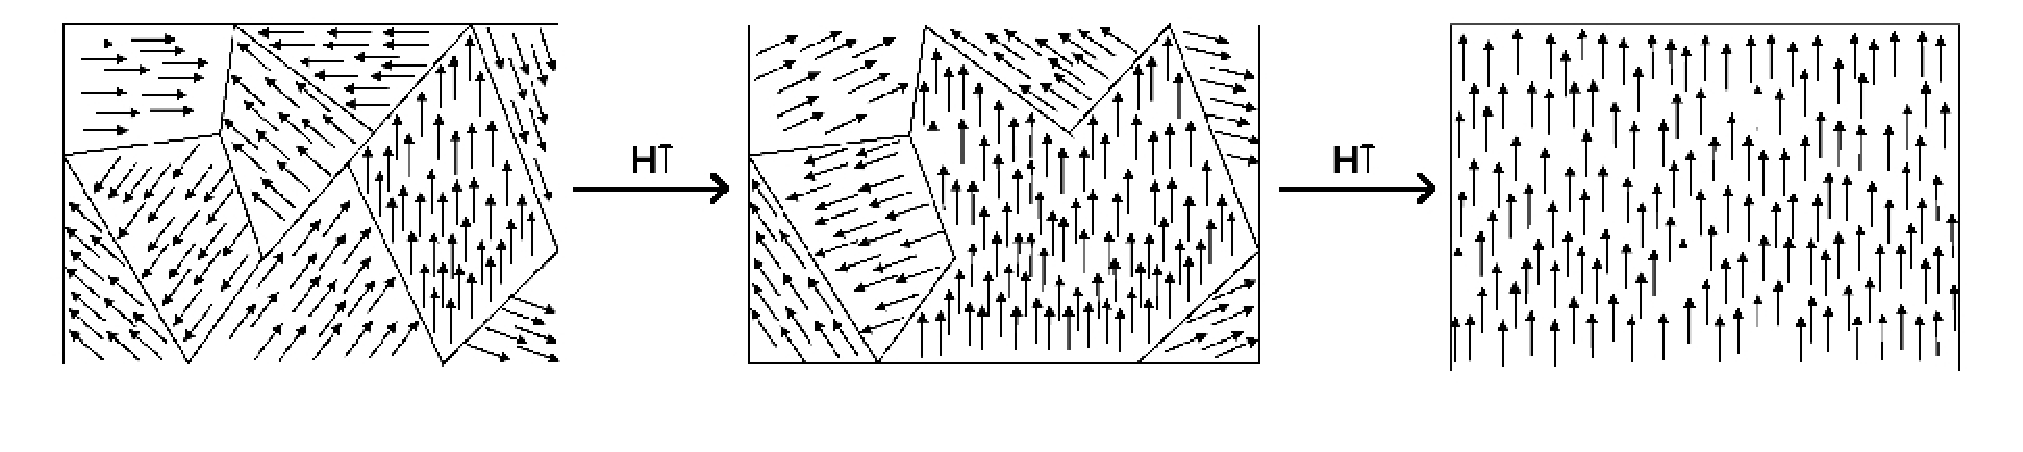
\includegraphics[width=0.9\linewidth]{img/Dominios.pdf}
        \end{center}
        \caption{
\small Rotation of orientation and increase in size of magnetic domains due to an externally applied field. Picture taken from \url{http://en.wikipedia.org/wiki/Magnetic_domain}.
        }
        \label{fig:doms}
\end{figure}

\subsubsection*{Magnetic Hysteresis}
Decreasing the external field after all domains were parallely oriented reverses the above effect and creates / enlarges domains with different orientation little by little. As the orientation flipping requires energy though, it will only happen, if the difference in total energy between the current and the flipped state is larger than this required energy. Thus there will be more domains with the original orientation, even after the external field has vanished. This remaining macroscopic magnetic moment is called the remanence magnetisation. An opposing field with the so called coercivity strength is required to completely demagnetize the material. The different magnetizations while increasing and decreasing the external field create the so called hysteresis curve (see figure \ref{fig:hys}).
\begin{figure}
        \begin{center}
         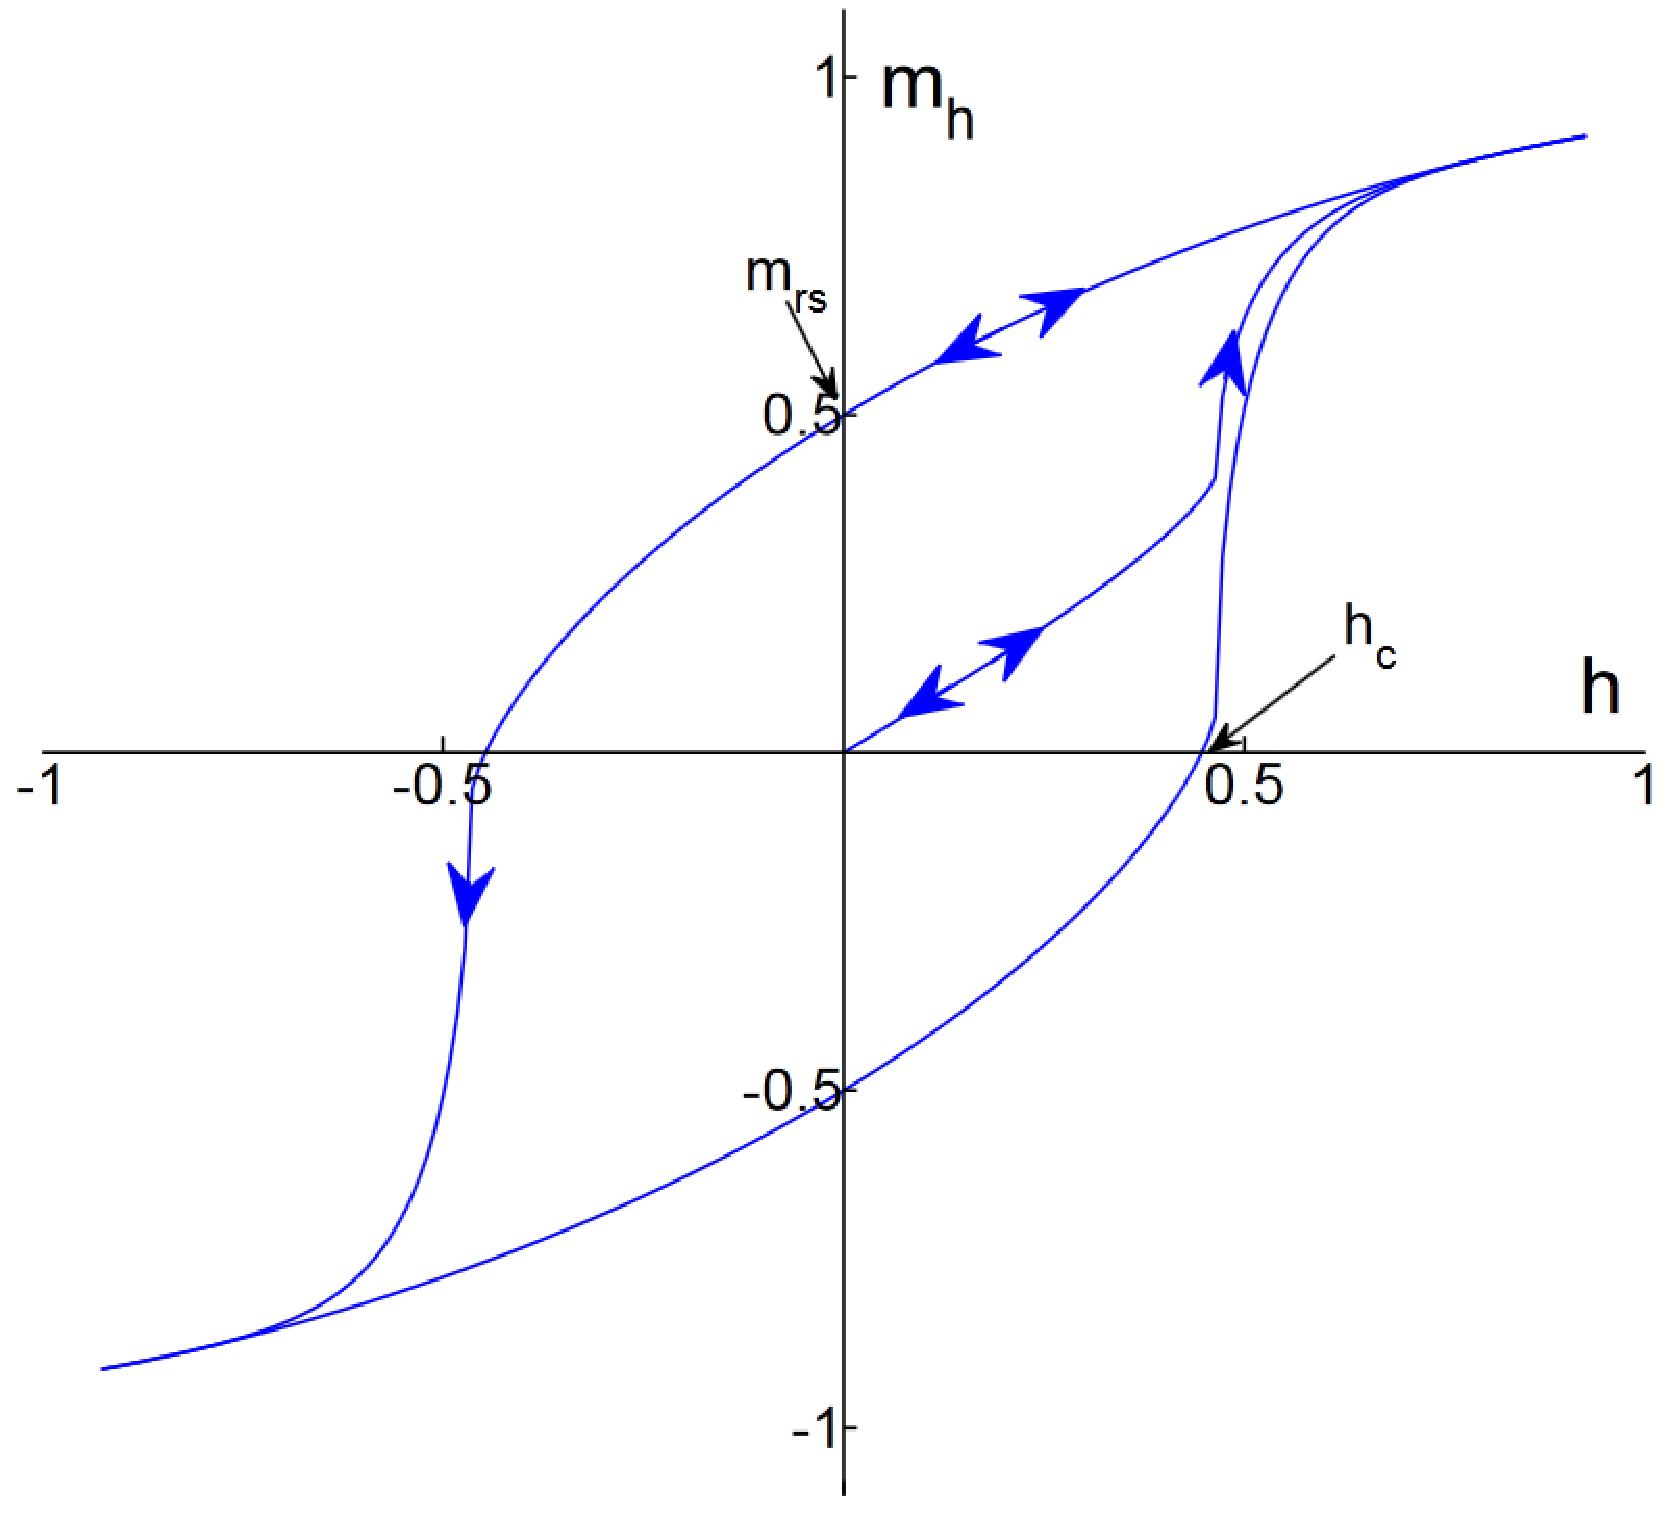
\includegraphics[width=0.31\linewidth]{img/hys.pdf}
        \end{center}
        \caption{
\small A plot of magnetization m against magnetic field h calculated using a theoretical model. Starting at the origin, the upward curve is the initial magnetization curve. The downward curve after saturation, along with the lower return curve, form the main loop. The intercepts $h_c$ and $m_{rs}$ are the coercivity and saturation remanence. Picture taken from \url{http://en.wikipedia.org/wiki/Hysteresis}.
        }
        \label{fig:doms}
\end{figure}


\subsubsection*{Magnetic Anisotropies}
A ferromagnet usually energetically prefers a certain direction of magnetization. This effect is called magnetic anisotropy and results mainly from two different contributions.

The shape of the magnetic sample is important as the stray field caused by the long range dipole-dipole interaction is dominated by the geometry of the sample. For thin films, the favorable magnetization direction lies within the plane of the film.

The other contribution is called the crystal anisotropy. It is a result of the spin-orbit interaction in every atom of the lattice and describes the fact that the magnetization direction along the different crystal axes result in different energy contributions. The crystal axes, which lead to minimal energy contribution are called "easy axes" in contrast to unfavorable axes, that are called "hard axes". For a small deviation of the angle $\Theta$ between the magnetization direction and the direction of the easy axis, the crystal anisotropy energy is given by
\eq{E_c=K \cos^2 \Theta \sin^2 \Theta \; , }{aniso}
where $K$ is the anisotropy constant in this lowest order approximation.


\section{Experimental Set-Up}
\subsection{Determination of Kerr Angle}
The rotation angle of the Kerr rotation is $\Phi_K$ and can be analyzed using a polarization filter, that is also called analyzer. While it is not possible to measure the rotation directly, the evolution of the intensity depending on the angle $\alpha$ is known to be
\eq{I(\alpha)=I_0 \cos^2(\alpha-\alpha_0) ,}{eq:malus}
where $\alpha_0$ is the angle of polarization. This equation as stated only holds for linearly polarized light, but in general circular or elliptically polarized light can be described as a superposition of two perpendicularly polarized light beams. The law thus becomes
\eq{I(\alpha) = I_0 \cos^2(\alpha-\alpha_0) + I_1 \sin^2(\alpha-\alpha_0) .}{}

It can be convenient to look at another value, that is useful to have at any rate: the contrast $c$. It is defined as the difference between minimum and maximum value devided by the offset (their average). In our case these minima and maxima are simply the intensities at the opposing saturation magnetisations.
\eq{c(\alpha)=\frac{\Delta I(\alpha)}{<I(\alpha)>} = 2\frac{I_+(\alpha)-I_-(\alpha)}{I_+(\alpha)+I_-(\alpha)} }{eq:contrast}
Where the two saturation intensities can be calculated by the above equation \Formel{eq:malus}
\eq{I_\pm(\alpha) = I_0 \cos^2(\alpha-\alpha_0\pm\Phi_K) + I_1 \sin^2(\alpha-\alpha_0\pm\Phi_K) }{}
where $\alpha_0$ now is the angle of the incident light. Combining this with \Formel{eq:contrast} results in
\eq{c(\alpha) = \frac{2(I_1-I_0) \sin(2(\alpha-\alpha_0)) \sin(2\Phi_K) } { I_0+I_1+ (I_0-I_1)\cos(2(\alpha-\alpha_0)) \cos(2\Phi_K)} .}{}



\subsection{Theoretical Calculation of Magnetic Field}
By the use of Ampere's Law, we obtain for a toroid coil with an iron core, that has radius $r$, winding number $n=300$ and a slit of width $d=\SI{12}{mm}$
\eq{nI=\oint_{\mathcal S} \vec{H} \cdot \mathrm{d}\vec{s} = 2 \pi r H_{Fe} + d H_{Air} \;, }{Htheo}
where $I$ is the current that runs through the coil. As the relative permeability for iron is by approximately a factor $3000$ higher then the permeability of air and the radius of the coil is not by orders of magnitudes larger than the slit width, we can neglect the first summand in \Formel{Htheo} yielding
\eq{B_{slit} =  \mu_0  H_{Air}= \frac{\mu_0 n}{d} I = \SI{31.4}{mT A^{-1}} I \; .}{}

 


 \bibliographystyle{unsrt}
\bibliography{FPbib}

\end{document}
